%!TEX encoding = UTF-8 Unicode
%!TEX program = arara
% arara: pdflatex: {synctex: yes}
%! arara: komkindex: {style: kotex}
% arara: pdflatex: {synctex: yes}
%%% file `kotexdoc.tex`
%% Written by Kangsoo Kim <karnes at ktug kr>
%%
%%  2013/09/30
%%  2013/11/07
%%  2014/03/01, \ksnamedef
%%
%% part of ko.TeX v2.0
%% LPPL, maintained.
%
\documentclass[a4paper,%
	10.5pt,%
	amsmath,%
%	uset1font,%
	chapter,%
	twoside,%
	openany,%
	finemath,%
	oldfontcommands]%
{oblivoir}

\usepackage{fancyvrb}
\usepackage{eurosym}

\ifPDFTeX
  \SetHanjaFonts{uhcmj}{nanumgt}{nanumgt}
  \usepackage[pdftex]{graphicx}
  \SetGremphFonts{nanumgt}{nanumgt}
  \usepackage[normalem]{ulem}
  \usepackage{dhucs-trivcj}
%  \usepackage{dhucs-midkor}
  \input sample-finemath-setup.tex
  \usepackage[T1]{fontenc}
  \renewcommand{\rmdefault}{nanummj}
\else
  \ifLuaOrXeTeX
  \usepackage{xob-dotemph}
  \setkormainfont(* ExtraBold)(*){NanumMyeongjo}(){HCR Batang LVT}
  \def\다{\nobreak 다}
\fi\fi

\usepackage[x11names,dvipsnames,svgnames]{xcolor}

\ifXeTeX
  \usepackage[normalem]{ulem}
\fi

\usepackage[dbl4x6]{fapapersize}
\usepackage{boxedminipage}

\SetHangulspace{1.5}{1.1}

\usepackage{hologo}
\def\pdfTeX{\hologo{pdfTeX}}
\def\pdfLaTeX{\hologo{pdfLaTeX}}
\def\XeTeX{\hologo{XeTeX}}
\def\XeLaTeX{\hologo{XeLaTeX}}
\def\eTeX{\hologo{eTeX}}
\def\LuaTeX{\hologo{LuaTeX}}
\def\LuaLaTeX{\hologo{LuaLaTeX}}
\usepackage{kotex-logo}

\newcommand*\kotex{\texorpdfstring{\textsf{k}\kern-0.0625em\textit{o}\kern-1.5pt\lower.15ex\hbox{.}\kern-1pt\protect\TeX}{ko.TeX}}
\def\ko{\textsf{k}\textit{o}}
\def\kotexplain{\kotex-\hologo{plain}}
\newcommand\kotexversion{v3.0}
%\newcommand\kotexdate{2013년 11월}
\newcommand\kotexdate{2021년 7월}

%\usepackage[
%    backend=biber,
%    style=authoryear,
%    sortlocale=UTF-8,
%    natbib=true,
%    url=true, 
%    doi=false,
%    eprint=false,
%]{biblatex}
%\addbibresource{kotexguide.bib}
%\addbibresource{texbook1.bib}
%\addbibresource{texbook3.bib}
%

\newenvironment{preamtext}{%
 \section*{제1판 일러두기}
}{\clearpage}

\newenvironment{preamtexttwo}{%
 \section*{제2판 일러두기}
}{\clearpage}

\newenvironment{preamtextthree}{%
 \section*{제3판 일러두기}
}{\par}

\def\util#1{\texttt{#1}\index{Utilities!#1}\index{#1}}
\def\pkg#1{\textsf{#1}\index{Packages!#1}}
\def\option#1{\texttt{[#1]}\index{Options!#1}}
\def\wi#1{#1\index{#1}}
\def\thispkg{\kotex}
\def\file#1{\texttt{#1}\index{Files!#1}}

\def\OMEGA{$\mathrm{\Omega}$}

\copypagestyle{part}{empty}

\renewcommand\cftsectionaftersnumb{\hspace{1.2em}}
\renewcommand\cftsubsectionaftersnumb{\hspace{1em}}

\def\xample{예시}
\renewcommand{\cmd}[1]{\cmdprint{#1}%
  \index{Commands!\string\cmdprint{\string#1}}}

\makeindex

\begin{document}

\frenchspacing

\title{한국어 텍 \kotex}
\author{김강수}
\date{version 3.0\quad\kotexdate}

\begin{titlingpage}
\maketitle
\end{titlingpage}

\frontmatter

\begin{preamtextthree}
2013년에 \koTeX 이 CTAN에 등재되어, 주요 \TeX{} 배포판에 수용됨에 따라
사실상 한국어 조판의 표준으로 자리잡은 지도 어언 수년이 흘렀다.
이 기간 동안 \koTeX 은 특히 \XeTeX 과 \LuaTeX 을 중심으로 크게 발전하여
2021년 현재 상업적인 출판에 무리없이 활용되어 높은 수준의 조판 품위를 보증할
정도가 되었음을 모두가 인정하고 있다.
저자들은 이를 매우 자랑스럽게 여기며, 버그 리포트와
중요한 기여, 그리고 일상적 격려를 통하여 이를 지원해준 사용자와 기여자 모두에게
깊은 감사를 표한다.

\koTeX{} 문서 제3판에서는 \koTeX-utf 매뉴얼 부분을 분리하였고
부분적인 가필과 수정을 행하였다. \koTeX-utf 사용법을 보려면 
\verb|texdoc kotex-utf|를 실행하라.

\bigskip

\hfill 2021년 7월 \par
\hfill 대표필자 김강수 (識)

\end{preamtextthree}
\begin{preamtexttwo}
2007년에 \kotex 이 만들어진 이후, 이 패키지는 사실상 한국어 문헌의
조판과 식자에 있어 가장 널리 사용되는 패키지가 되었습니다.
저자들은 이에 대해 매우 자랑스러움을 느끼고 있으며, 개선을 위해 고언을
마다하지 않으신 사용자 여러분께 깊이 감사드립니다.

2007년 이후, 텍 사용환경에는 극적이라 해도 좋을 만한 변화가 초래되었습니다.
특히 \XeTeX 이나 \LuaTeX 과 같은 새로운 엔진이 등장하여,
한글 식자 문제에 있어 결정적인 진보를 이룬 것은 특기할 만한 것입니다.
\kotex 의 저자들은 이와 같은 텍 환경 변화에 발맞추어 \XeTeX-\ko, \LuaTeX-\ko와 같은 패키지를 개발하여 한글 사용을 더 쉽고 강력하게 만드는 데 헌신해왔습니다.

이에 2013년에 접어든 지금, \kotex 을 전반적으로 정비하고 그 사용 설명서를
작성하게 되었습니다. \kotex 은 더 발전할 것이고, 더 훌륭한 한글 문헌의
조판을 가능하게 할 것입니다.

이 문서가 조금이라도 도움이 되기를 바랍니다.

\bigskip

\hfill 2013년 9월 

\hfill (대표필자) 김강수 (識)

\end{preamtexttwo}


\begin{preamtext}
\kotex 은 H\LaTeX 과 hangul-ucs가 결합하여 탄생한, 명실
상부한 ``한국어(한글) 텍 시스템''입니다. ``한글 라텍(H\LaTeX)''은 1990년대 이후
텍에서의 한글 사용에 \dotemph{사실상 표준}이었으며, hangul-ucs는
한글 라텍의 현저한 영향 아래서 성장한 유니코드 한글 텍 매크로였던 것입니다.

이제 한국텍학회(KTS)의 주도 아래, 한글 라텍과 hangul-ucs가
하나의 매크로 시스템으로 통합된 것을 매우 기쁘게 생각합니다.
이와 더불어 더욱 알차고 유용한 사용자 안내서를 작성하기 위해
많은 노력을 하였습니다.

한글 라텍의 표준 문서였던 ``한글 라텍 길잡이''(\wi{은광희})는 아마도 가장 많이
읽힌 한글로 된 라텍 관련 문서 중 하나가 아닐까 합니다. 이 문서는 단순히 한글
사용법을 넘어서서, 텍에 입문하는 데 있어서도 많은 도움을 주었습니다.

이 문서는 한글 라텍 길잡이를 바탕으로 \kotex 에 맞도록 개정하여
쓴 것입니다. 감사의 말과 머리말은 거의 그대로 보존하였으며, \kotex 이
등장하는 경과를 설명하는 소절을 하나 추가하는 정도에 그쳤습니다.
다만 문체의 일치를 유지하기 위하여 이 일러두기와 감사의 말을 제외하고는
경어체를 평어체로 고쳐썼습니다. 또한
사용법에 있어서 한글 라텍 이후의 여러 가지 발전 사항을 새로운 편제로
서술하려 하였습니다. 지나치게 기술적인 서술을 피하고 실제 사용자에게
구체적인 지침을 제공하는 데 이 문서의 목적이 있습니다. 

이 문서가 \kotex 을 사용하는 분에게 조금이라도 도움이 되기를 바랍니다.
뜻하지 않은 잘못된 내용이나 실수, 빠진 내용, 오식을 바로잡아 주시면 더 나은
사용자 안내서를 만드는 데 크게 도움이 될 것입니다. 

\bigskip
\rightline{2007년 7월}
\rightline{\wi{은광희} \wi{김도현} 김강수 (識)}

\end{preamtext}

\tableofcontents*


\mainmatter
\pagestyle{hangul}

%\part{총론}

\chapter{\kotex 에 관하여}

\section{\kotex 의 구성}

\kotex\footnote{\kotex은 텍스트
  상황에서 \texttt{ko.TeX}이라고 쓰고 ``케이오텍'' 또는
  ``코리언 텍''이라고 읽는다. ``코텍'' 또는 ``코텍스''라고
  읽지 않기를 희망한다.
  \texttt{ko}는 한국어를 의미하는
  국제부호에서 취한 것이다. \texttt{ko}를 소문자로 쓴다.}%
은 한국어/한글 식자를 위한 \hologo{plainTeX}, \LaTeX\ 패키지군을 아울러 부르는 말이다.
\wi{한국텍학회}(KTS; Korean \TeX\ Society)에서 공식적으로 개발을 후원하고 배포를 담당하고 있으며,
핵심 기능의 주개발자인 \wi{김도현} 이외 많은 기여자들이 개발에 참여하고 있다.

2021년 현재, \kotex 과 그 관련 패키지의 목록은 다음과 같다.
\begin{enumerate}[(1)] \oblivoirlist
\item \textbf{\kotex-plain}. \TeX 과 \LaTeX 에서 한글을 구현하기 위한
핵심 매크로들과 \hologo{plainTeX}을 위한 스타일로 이루어져 있다.
\item \textbf{\kotex-utf}. \eTeX, \pdfTeX\ 엔진 위에서 운영되는
\LaTeX 에서 한글을 구현한 패키지이다. 은광희의 H\LaTeX 의 계보를 잇는
\LaTeX\ 한글 패키지로서, H\LaTeX\ 스타일의 장절표제를 위한 \pkg{kotex-sections}를
포함하고 있다.
\item \textbf{cjk-\ko}. \eTeX, \pdfTeX\ 엔진 위에서 운영되는
\LaTeX 을 위한 한글 패키지이며, \kotex-utf와 달리 Werner Lemberg의 \pkg{CJK} 패키지를
이용하고 있다. 
\item \textbf{\XeTeX-\ko}. \XeTeX\ 엔진에 대응하는 한글 조판 패키지이다.
\item \textbf{\LuaTeX-\ko}. \LuaTeX\ 엔진에 대응하는 한글 조판 패키지이다.
\item \textbf{\koTeX-oblivoir}. \pkg{memoir} 클래스로 한글을 조판하기 위한 클래스와
패키지의 묶음이다.
\item \textbf{\koTeX-utilities}. 한글 처리에 필요한 유틸리티. 색인을 만들기 위한
\util{makeindex}의 한글판 \util{komkindex}, \util{xindy}의 한글 모듈,
그리고 \util{jamo-normalize} 등을 포함한다.
%\item \textbf{\kotex-utf}. 유니코드 (UTF-8) 한글
%식자 패키지로서, ``legacy \TeX\ 엔진'' ({\small \util{tex}, \util{latex}, \util{pdftex}, \util{pdflatex}을 실행하는 경우 운용되는 \TeX\ 엔진})에
%대응한다. \LaTeX 을 위한 \pkg{dhucs}와 \hologo{plainTeX}을 위한 \pkg{kotexplain}, 그 부수파일들로 이루어져 있다.\index{dhucs}
%\item \textbf{cjk-\ko}. Werner Lemberg의 \pkg{CJK} 패키지를 이용하여
%유니코드 한글을 식자하는 패키지이다. legacy \TeX\ 엔진에 대응한다.
%이 패키지는 그 기원과 동작이 \kotex 과는
%제법 다르게 출발하였지만 \kotex 의 몇 가지 중요한 기능\explpunc.자동조사 등.\ 을 구현하고 있는 등, 여러 면에서 \kotex 의 일부로 간주할 수 있다.
%\cmd{\usepackage\{kotex\}} 문법을 사용한다.
%\item \textbf{\XeTeX-\ko}. \XeTeX\ 엔진에 대응하는 한글 식자 패키지이다.
%\item \textbf{\LuaTeX-\ko}. \LuaTeX\ 엔진에 대응하는 한글 식자 패키지이다.
%\item \textbf{oblivoir}. \pkg{memoir} 클래스를 이용하여 한글 문서를 작성하도록 도와주는 클래스와 패키지 묶음이다. 
%\item \textbf{\kotex\ utilities}. 한글 문서 작성에 필요한 유틸리티들이다.
%예를 들면 색인을 만들기 위한 \util{komkindex}와 \util{xindy modules} 등이 포함되어 있다.
\end{enumerate}

위에 열거한 한글 패키지들은 모두 원칙적으로 유니코드(UTF-8) 한글을
처리하는 것이다. 소위 `완성형 한글'을 지원하던 H\LaTeX 과 \koTeX-euc는
현재 ``개발 중단(obsolete)'' 상태로 간주되며, 개발이 그친 상태 그대로
별도로 보존되고 있다. 

\TeX\,Live로 배포하는 CTAN 등재 한글 글꼴 패키지가 있다. 

\begin{enumerate}[(1)]\oblivoirlist
\item \textbf{nanumtype1}. 나눔명조와 나눔고딕 글꼴(원본은 트루타입)을 레거시
텍에서도 쓸 수 있도록 \TeX\ 폰트로 변환한 글꼴 묶음이다. Type 1 포맷이며, TFM과
FD 파일을 함께 제공한다. 패키지의 관리자는 김도현이다.
\item \textbf{uhc}. 은광희의 H\LaTeX\ 기본 폰트였던 mf, type 1 글꼴이다. \koTeX-utf는
명조체 한자 글꼴을 이 폰트를 이용하여 식자한다.
\item \textbf{unfonts}. 은광희의 UHC 폰트를 트루타입으로 변환한 글꼴이다.
드물게 보는 완전한 자유 한글 글꼴이며, \koTeX 의 개발 단계에서 사실상의
표준 글꼴로 간주되었던 적이 있다. 현재 CTAN에 등재되어 트루타입 형식 그대로
\XeTeX 과 \LuaTeX 에서 활용할 수 있다. \util{unfont-core}와 \util{unfonts-extra}라는
두 개의 패키지로 등록되어 있다.
\item \textbf{baekmuk}. 김정환의 백묵 글꼴로서, 저작권 관련 문제가 해결된
후에 CTAN에 등재되었다.
\end{enumerate}

%다음 패키지는 이전 버전까지 \kotex 에 포함되어 있던 것들이나, 2.0 버전에서
%제외되어 현재 ``개발 중단(obsolete)'' 상태로 간주되는 것들이다. 이 패키지들은
%편의를 위하여 현재까지 \kotex\ 저장소에서 서비스하고 있다.
%\begin{enumerate}[(1)]
%\item \textbf{kotex-euc}. EUC-KR 한글을 식자하는 패키지였다.
%\wi{은광희}의 H\LaTeX\ 1.0.1의 \LaTeX\ 파트를 바탕으로 약간의 수정을 가한 상태로
%\kotex\ 1.0에 포함되어 있었다.
%\item \textbf{untype1}.\index{은글꼴 type 1} 은글꼴 type 1 폰트 묶음이다. 역시 ``개발중단''
%상태이고 \kotex\ 2.0에서는 불필요하나 이 글꼴 묶음을 필요로 하는 분이 계실 것을 감안하여 당분간 
%\kotex\ 저장소를 통하여 제공받을 수 있다.\footnote{참고로, 그동안 \kotex 은 편의를 위하여
%	은글꼴 트루타입도 함께 배포해왔으나, 이것은 원래부터 \kotex 의 일부는 아니었고 단지
%	은글꼴 트루타입을 기본 글꼴로 간주한 패키지가 존재했던 데서 연유한다.}
%\item \textbf{kotex-euc-utils}. \pkg{kotex-euc} 패키지에 딸려 있는
%유틸리티들이다. \util{hmakeindex}와 \util{hbibtex}으로 이루어져 있다.

%이밖에 \kotex 의 일부는 아니지만 이와 밀접한 관계를 갖고 있는 패키지는 다음과 같다.
%\begin{enumerate}[(1)]
%\item \textbf{nanumtype1}. CTAN에 등록되어 있는 (유니코드) 한글 type 1 글꼴이다. 패키지의 관리자는 \kotex 의 주개발자인 \wi{김도현}이다.
%\end{enumerate}

%\begin{figure}
%\centering
%\includegraphics[width=.95\linewidth]{fig/whatkotexconsistof}
%\caption{\protect\kotex 의 연혁과 구성}\label{fig:consistsof}
%\end{figure}

\section{간단한 연혁}

\subsection{\protect\kotex 의 탄생 (2007)}

\begin{figure}[t]
\centering
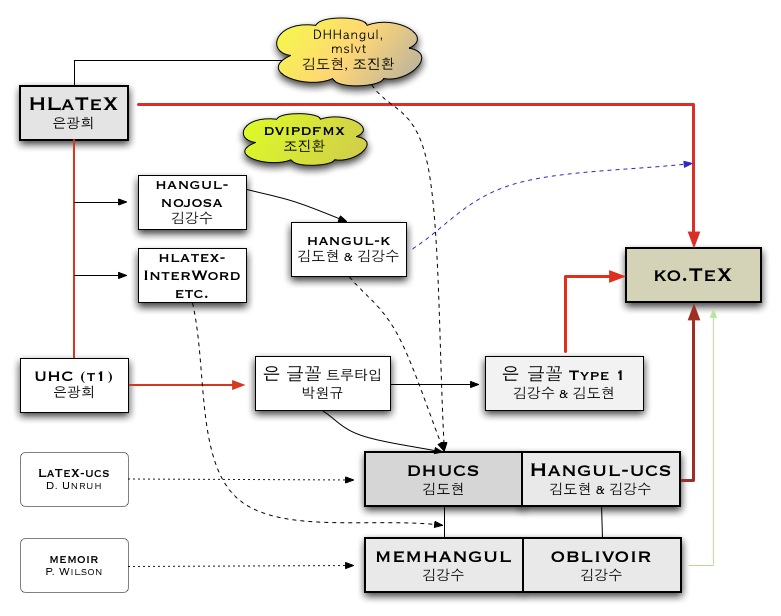
\includegraphics[width=\linewidth]{fig/histkotex}
\caption{\protect\kotex 의 탄생}\label{fig:hist}
\end{figure}

그림~\ref{fig:hist}\는 H\LaTeX 에서 출발하여 \kotex 에 이르는
한글 텍의 발전 과정을 요약한 것이다. 

2007년 6월 30일, 한국텍학회 모임에서, \wi{은광희}\cntrdot \wi{김도현}\cntrdot 김강수 등
한글 라텍 및 hangul-ucs의 저자들과 KTS 임원\cntrdot 회원 등이 모인 자리에서
이 두 한글 매크로 패키지를 통합하여 \wi{통합 한글 텍 패키지}를 제작하기로
의견을 모은 것이다. 이것은 그동안 한글 사용에 있어서 둘 이상의 패키지가
존재함으로 인해 빚어진 혼란을 불식하고 향후 한글 텍/라텍의 발전의
근거를 마련했다는 점에서도 중요한 일보전진이었고, 한글 라텍으로부터
오랜 시간 발전해 온 라텍에서의 한글 사용을 총체적으로 점검할 기회를
얻게 되었다는 점에서도 의미가 있는 결정이었다.

그로부터 일 개월 정도의 작업을 통하여 \kotex\ 베타 버전이 공개되었다.
\kotex 은 Unicode/UTF-8 인코딩과 EUC-KR을 모두 지원하기로 하였으나
원칙적으로 향후의 발전 방향은 Unicode로 합의하였다. 또한 \wi{은광희}의
UHC 글꼴을 발전시킨 `은글꼴 type 1'을 기본 글꼴로 채택하고 이를
EUC-KR 버전에도 적용시킴으로써, 폰트를 둘러싼 이런저런 불편한 점을
일소하였으며, pdf 제작 및 매크로의 호환성과 안정성에 있어서
몇 가지 중요한 진보를 이루었다.

\subsection{그 후의 발전}

\kotex 은 \TeX\,Live\index{TeX Live}에 대응하여 개발되기 시작하였다. 2008년부터
\TeX\,Live의 사설 저장소를 만들고 이를 통하여 \kotex 을 배포해왔다.
이 시기의 중요한 사실을 요약하면 다음과 같다.
\begin{itemize}
\item KTUG을 통해 이루어진 Hanyang PUA project의 결과, 고문헌
조판에 필요한 유틸리티를 갖추게 되었다.
\item \XeTeX-\ko와 \LuaTeX-\ko가 개발되었다.
글꼴의 제약이 사라짐으로써 누리게 된 이점 때문에 사실상 \XeLaTeX 을
한글 문헌 조판에서 본격적으로 사용하게 되었다. 이에 더하여 \pkg{oblivoir}의 \XeTeX 판인 \pkg{xoblivoir}가 별도로 개발되었다.
\item \pkg{cjk-ko}, \pkg{nanumtype1}, \pkg{luatexko}, \pkg{xetexko}가 \TeX\,Live를 통해 배포되기 시작하였다.
\end{itemize}

현재 한글 문헌을 가장 안정적으로 조판할 수 있는 것은
\XeTeX-\ko이다. \LuaTeX-\ko는 실험적인 성격이 강하고,
레거시 텍을 위한 \kotex-utf는 하위호환성이나 특수한 상황\footnote{%
	모바일 기기에서 텍을 이용한다든가 하는 상황. 특히 \pkg{cjk-ko}는 
	이러한 목적을 위하여 개발되었다.}%
을 위하여
필요로 하는 정도가 되었다.
특히 유니코드 텍 엔진의 등장은 \kotex 을 개발하면서 직면했던 많은 고민들,
예컨대 글꼴 사용의 문제 같은 것을 일소할 수 있게 하였다.

\section{\kotex 의 로고}

\kotex 의 로고는 다음과 같다.
\begin{center}
\LARGE\kotex
\end{center}
\begin{boxedverbatim}
\newcommand*\koTeX{%
  \textsf{k}\kern-0.0625em\textit{o}\kern-0.11em%
  \lower.15ex\hbox{.}\kern-0.1em\protect\TeX}
\end{boxedverbatim}
이 로고는 \kotex 의 견고함과 아름다움, 그리고 유연한 표현능력을 상징한다.
\pkg{kotex-logo} 패키지에 정의되어 있으므로 \cmd{\usepackage\{kotex-logo\}}를
선언하면 \cmd{\koTeX} 명령을 쓸 수 있다.

\section{개발자와 라이선스}

\kotex 의 주개발자는 다음과 같다. 개발자는 LPPL의 maintainer를 겸한다.
\begin{description}\tightlist
\item [\kotex-utf] \wi{김도현}, 김강수 (LPPL, maintained)
\item [\XeTeX-\ko] \wi{김도현} (LPPL, maintained)
\item [\LuaTeX-\ko] \wi{김도현} (LPPL, maintained)
\item [cjk-\ko] \wi{김도현} (GPL, LPPL)
\item [oblivoir] 김강수, 이기황 (LPPL, maintained)
\item [\kotex-euc] \wi{은광희}, \wi{김도현}, 김강수 (obsolete)
\item [untype1]\index{은글꼴 type 1} \wi{은광희}, \wi{박원규}, \wi{김도현}, 김강수 (obsolete)
\end{description}

\pkg{untype1}과 \pkg{cjk-ko}의 일부 파일을 제외한 모든 패키지가 LPPL 라이선스를 가진다.\footnote{참고로, untype1은 GPL이다.}

\chapter{kotex.sty}

\section{패키지 사용 선언}\label{sec:kotexsty}

\kotex\ 전체를 통틀어 \pkg{kotex}이라는 패키지를 부르는 것으로
한글 사용을 선언할 수 있다.
이 패키지는 현재 동작하는 \TeX\ 엔진과 주어진 옵션에 따라 적절한
\kotex\ 패키지를 불러오는 wrapper 역할을 한다.

\begin{boxedverbatim}
\usepackage[<options>]{kotex}
\end{boxedverbatim}

줄 수 있는 옵션은 실제 호출되는 한글 패키지의 기능과 동작에 따라 조금씩 다르지만, \option{hangul}
옵션은 특기할 만하며, 문서의 줄 간격, `이름' 등을 한글화한다.
\option{hanja}도
이와 비슷한데, 기본적으로 \option{hangul}을 적용한 후에 캡션 등을
한자화한다.
이 두 옵션은 모든 \kotex\ 패키지군에 공통적으로 적용된다.

\begin{table}
\centering
\caption{실제로 동작하는 \kotex\ 패키지}\label{tab:engines}
\begin{tabular}{c|c|c}
\hline
\cmd{\usepackage} & 대응 엔진 & 동작하는 패키지 \\ \hline \hline
\cmd{[cjk]\{kotex\}} & \pdfLaTeX & \pkg{cjkutf8-ko} \\ \hline
\cmd{...\{kotex\}} & \pdfLaTeX & \pkg{dhucs} \\ \hline
\cmd{...\{kotex\}} & \XeLaTeX & \pkg{xetexko} \\ \hline
\cmd{...\{kotex\}} & \LuaLaTeX & \pkg{luatexko} \\ 
\hline
\end{tabular}
\end{table}

\tref{tab:engines}에서 보는 바와 같이 동일한 호출 명령을 주어도
실제로 동작하는 한글 패키지가 어떤 것이냐 하는 것은 실행되는
텍 엔진과 옵션에 따라 달라진다.

\section{\protect\pdfLaTeX\ 또는 \LaTeX 으로 컴파일}

\noindent\cmd{\usepackage[cjk]\{kotex\}}

위와 같이 \option{cjk}가 주어지면 \pkg{cjk-ko} 패키지를 부른다.
정확하게는 \pkg{cjkutf8-ko.sty}라는 파일을 불러온다.
%추가할 수 있는 동작은 \option{hangul}, \option{hanja},
%\option{nojosa}라는 공통 옵션 이외에 \option{usedotemph},
%\option{usecjkt1font}가 있다. 각각의 의미와 동작에 대해서는
%\Cref{chap:docu}에서 언급한 문서를 보라.

\bigskip

\noindent\cmd{\usepackage[utf]\{kotex\}}

\koTeX-utf 패키지로 한글을 처리한다. 이것이 기본값이다.
%\pkg{dhucs.sty}를 찾는다. 이것이 기본값이며, 
%이 문서의 제\,\ref{part:two}\,편에서 설명하는 것이 이 경우의
%문서 작성법이다.
%\XeTeX과 같은 새로운 엔진이 등장하기 전에 
%\kotex 이라 하면 \pkg{dhucs}를
%통하여 \pdfLaTeX 으로 한글을 식자하는 것을
%일컫는 것이었다.
%기본값이므로 \option{utf}를 지정하지 않아도 된다.
%추가 옵션에 대해서는 이 문서의 해당 부분(제\,\ref{part:two}\,편)을 참고하라.

\section{\XeLaTeX\ 또는 \LuaLaTeX 으로 컴파일}

각각 \pkg{xetexko.sty}와 \pkg{luatexko.sty}를 찾는다.
즉 \cmd{\usepacakge\{kotex\}}을 지정하는 것은 동일하지만
\util{xelatex}으로 문서를 컴파일한다면 전혀 다른 패키지를 사용하는 
것인 셈이다.

이 엔진과 패키지를 사용하는 것은 종래의 \pdfLaTeX 으로 작업하는 것과는
몇몇 부분이 다르다. 따라서 해당 문서를 잘 읽고 이에 대응해야 한다.
그러나 \option{hangul}, \option{hanja} 옵션은 여전히
비슷한 의미로 동작한다.

\section{엔진별 동작의 예시}

어떤 문서를 작성하였고, 어떤 엔진으로 컴파일될지 모르는 상황이라면
되도록 호환성있게 원본 자체를 작성하면 좋을 것이다.
이럴 때 요긴하게 쓸 수 있는 패키지로 \pkg{iftex}이 있다.
다음 보기는 이러한 상황에 대응하는 한 가지 예이다. (cjk-\ko를 이용하는
경우는 예시에서 제외되었다.)

\begin{boxedverbatim}
\documentclass{article}

\usepackage[hangul]{kotex}

\usepackage{iftex}
\ifPDFTeX
  \usepackage{dhucs-nanumfont}
\else\ifXeTeX
  \setmainhangulfont{NanumMyeongjo}
\else\ifLuaTeX
  \setmainhangulfont{NanumMyeongjo}
\fi\fi\fi
\end{boxedverbatim}

%\section{pdf 문서 작성을 위한 설정}\label{sec:makepdf}
%
%%\subsection{pdf bookmark}
%%
%%%\paragraph{pdf bookmark}
%%
%%\pkg{hyperref}에
%%\option{pdfencoding = auto} 옵션을 지정하는 것으로 pdf bookmark 문제가
%%모두 해결된다.\footnote{%
%%	과거 \XeTeX 을 사용할 때는 \option{unicode} 옵션을 선언하지
%%	않고 \LuaTeX 이나 \pdfTeX 에서는 \option{unicode}를 선언하도록
%%	권장했다. 이 방법은 여전히 유효하나 \option{pdfencoding=auto}를
%%	쓰면 엔진에 따라 옵션을 달리 주어야 할 필요가 없다.}
%%\begin{verbatim}
%%\usepackage{kotex}
%%\usepackage{pdfencoding=auto,bookmarks]{hyperref}
%%\end{verbatim}
%%%여기서는 \option{unicode} 옵션이 반드시 지정되어야 한다.
%%%\option{pdftex}은 컴파일 상황에 따라 \option{dvipdfmx}
%%%또는 \option{dvips}를
%%%지정할 수 있다.
%%%
%%%위의 예에 상당하는 컴파일 절차 예시는 다음과 같다.
%%%\begin{verbatim}
%%%$ (pdf)latex foo
%%%$ (pdf)latex foo
%%%$ (dvipdfmx foo)
%%%\end{verbatim}
%
%\subsection{텍스트 검색과 추출}
%pdf 문서의 텍스트 검색과 추출은 매우 중요한 문제이다.
%이것은 어떤 드라이버로 pdf를 생성하느냐에 따라 조금 달라지는데, 일괄
%요약하면 다음과 같다.
%\begin{description}
%\item[dvipdfmx] type 1 글꼴을 매우 잘 처리하고
%이로부터 검색 및 추출이 가능한 pdf를 만들어낸다. 별도의 조치가
%필요없다.
%\item[dvips] 트루타입을 처리하지 못하는 점 때문에 이전부터
%문제가 있다고 생각되었으나 type 1 폰트를 사용하는 한
%검색 추출에 문제는 없다. 역시 별도의 조치가 필요없다.
%\item[pdftex] 이때는 \cmd{\pdfgentounicode}를
%활성화해주어야 한다.
%\end{description}
%그러므로 \wi{전처리부}(preamble)\explpunc.\cmd{\begin\{document\}} 명령이 놓이기 전.\ 에 다음과 같이 선언하는 것으로 충분하다.
%\begin{verbatim}
%\ifpdf
%  \input glyphtounicode
%  \pdfgentounicode=1
%\fi
%\end{verbatim}
%
%어떤 드라이버를 사용하든 모두 포스트스크립트 윤곽선 글꼴이 사용되고,
%pdf 북마크가 잘 만들어지며 한글 텍스트의 검색과 추출이 자유롭다.
%
%\paragraph{oblivoir}
%\pkg{oblivoir}는 위의 절차를 모두 자동화해두었다.

%\subsection{\LuaTeX, \XeTeX}
%
%이 엔진을 사용하는 경우, 기본 output이 pdf 포맷이다.
%pdf bookmark의 경우만이 문제가 되는데, \pkg{hyperref}을 사용할 때
%\begin{verbatim}
%pdfencoding = auto
%\end{verbatim}
%옵션을 쓰면 \pdfTeX, \XeTeX, \LuaTeX 을 불문하고 책갈피에서 한글이 깨지지 않게 해준다.
%
%과거에는 \XeTeX\ 사용시에 \option{unicode} 옵션을 주지 않아야 하는 데 
%주의해야 했으나 위와 같이 하면 자동적으로 처리된다.

\chapter{문서와 도움말}\label{chap:docu}

\koTeX 은 컴파일 엔진에 따라 동작하는 패키지가 다르다.
각각의 패키지는 별도의 사용안내서가 마련되어 있다.
그러므로 사용법에 대한 안내를 얻으려면 각 패키지별 문서들을 참조하여야 한다.
문서를 읽을 때는 \TeX\,Live 유틸리티 \util{texdoc}을 이용한다.
이 문서 자체는 명령행에서 \cmd{texdoc kotex}으로 읽을 수 있다.

\begin{description} 
\item [\kotex-utf] kotex-utf-doc 문서를 찾아 읽는다. 명령행에서 \cmd{texdoc kotex-utf} 
명령을 내려 읽을 수 있다.
\item [cjk-ko] cjk-ko-doc 문서를 찾아 읽는다. 명령행에서 \cmd{texdoc cjk-ko} 명령을 내리면 읽을 수 있다.
\item [\XeTeX-\ko] xetexko-doc 문서를 찾아 읽는다. 명령행에서 \cmd{texdoc xetexko} 명령을 내리면 읽을 수 있다.
\item [\LuaTeX-\ko] luatexko-doc 문서를 찾아 읽는다. 명령행에서 \cmd{texdoc luatexko} 명령을 내리면 읽을 수 있다.
\item [oblivoir] memoir 안내서를 보아야 한다. 이것은 
\cmd{texdoc memman} 명령으로 읽을 수 있다.. 한편, 한글화 부분에 대한 사항을 참고하려면 \cmd{texdoc ultrasimple} 명령으로 볼 수 있는 문서를 참고한다.
\end{description}

%%2.0 버전에서 제외된 패키지들을 굳이 사용할 필요가 있을 때,
%\kotex-euc와 \pkg{untype1}의
%사용법을 알려면 다음 문서를 참고하라.
%
%\begin{description}
%\item [kotexguide] \kotex\ 0.1.0 사용자 설명서이다.
%특히 \kotex-euc\index{Packages!kotex-euc}와 \pkg{untype1}\index{은글꼴 type 1}에 관한 방대한 사용 설명이 존재한다.
%\pkg{kotex-euc}를 설치하면 포함되어 있다.
%\end{description}


\chapter{배포와 설치}

\section{CTAN을 통한 배포}
%현재 \kotex 은 
%\begin{enumerate}[(1)]
%\item \wi{CTAN}\footnote{\url{http://ctan.tug.org}}에 등재
%\item \kotex\ 사설 저장소\footnote{\url{http://ftp.ktug.org/KTUG/texlive}}를 통하여 배포
%\end{enumerate}

현재 \kotex\ 패키지군은 거의 모두
CTAN에 등재되었다. CTAN을 통해 배포되는 패키지는 다음과 같다:
\begin{quote}
\pkg{kotex-utf}, \pkg{xetex-ko}, \pkg{luatex-ko},
\pkg{cjk-ko}, \pkg{kotex-oblivoir}, \pkg{kotex-utils},
\pkg{kotex-plain}, \pkg{nanumtype1}
\end{quote}

이 가운데, \pkg{kotex-plain}, \pkg{cjk-ko}, \pkg{xetex-ko},
\pkg{kotex-utf}는 서로 필요로 하는 파일이 의존되어 있어 함께
설치하는 것이 좋다. \pkg{luatex-ko}에서도 \pkg{xetex-ko}에서
필요한 파일을 찾을 때가 있다.

\hologo{pdfLaTeX}을 사용하려면 (다른 폰트를 설치하지 않은 경우) \pkg{nanumtype1}이 필요하다. 이 역시
CTAN을 통해 배포된다.

%\kotex\ 패키지군 가운데 2013년 11월 현재 CTAN에 등재되어 있는 것은
%\pkg{cjk-ko}, \pkg{xetexko}, \pkg{luatexko}, 세 종류이다.
%이들은 \TeX\,Live\index{TeX Live} 배포판에도 포함되어 있다.
%\pkg{nanumtype1} 패키지 역시 그러하다.

%\kotex\ 사설 저장소에는 이보다 많은 패키지가 서비스되고 있다. \kotex-utf의
%매크로와 유틸리티도
%이곳에서 배포된다.\footnote{%
%	멀지 않은 장래에 \pkg{dhucs}, 즉 \kotex-utf도 CTAN을 통하여 배포될 전망이다.}

CTAN에 등재된 패키지들은 각 배포판의 패키지로서 배포된다. \TeX\,Live와
MiK\TeX 에 \koTeX 이 모두 포함되어 있다.

\TeX\,Live는 한글 관련 패키지와 유틸리티, 문서를 \pkg{collection-langkorean}이라는 콜렉션 패키지로 묶어서 배포한다.

\section{github 저장소}

\begin{itemize} \oblivoirlist
\item \textbf{kotex-plain} \url{https://github.com/kihwanglee/kotex-plain}.
\item \textbf{kotex-utf} \url{https://github.com/kihwanglee/kotex-plain}.
\item \textbf{kotex-utils} \url{https://github.com/kihwanglee/kotex-utils}.
\item \textbf{kotex-oblivoir} \url{https://github.com/kihwanglee/kotex-oblivoir}.
\item \textbf{xetexko}. \url{https://github.com/dohyunkim/xetexko}.
\item \textbf{luatexko}. \url{https://github.com/dohyunkim/luatexko}.
\item \textbf{cjk-ko}. \url{https://github.com/dohyunkim/cjk-ko}.
\end{itemize}

\section{KTUG 사설 저장소}

과거 \kotex 이 CTAN에 등재되기 전에 KTUG은 \kotex\ 사설 저장소를 운영하여 \TeX\,Live에서의 설치를 지원하였다(2008--2013).

현재 사설 저장소는 CTAN에 등재하면서 제외된 \kotex-euc 파트와 은 글꼴(트루타입, type1) 및 KTUG에서 제작된 유용한 패키지와 유틸리티들을 추가적으로 서비스하는 목적으로 운영되고 있다. 
%에서 서비스되는 패키지는 \pkg{kotex-base}, \pkg{kotex-extra}, \pkg{jiwonlipsum}, \pkg{kotex-midkor}, \pkg{kotex-euc}인데 필수적인 패키지는 모두 CTAN으로 올라갔고 \kotex 의 기능을
%확장하는 보충적인 패키지들이 사설 저장소를 통하여 제공되고 있다.

%CTAN에 등재된 패키지들은 \TeX\,Live, MiK\TeX\ 등의 텍 배포판에
%포함될 수 있다. 따라서 \TeX\,Live를 설치한 경우 별도의 추가 작업 없이도
%\kotex\ 관련 패키지를 설치 운영할 수 있게 되는 것이다.

사설 저장소는 파일들을 몇 가지 ``설치용'' 패키지로 나누어서 제공한다.
2014년 5월 현재 사설 저장소를 통하여 설치할 수 있는 것은 다음과 같다.\footnote{%
	여기서 `패키지'란 \LaTeX\ 매크로 패키지를 가리키는 것이 아니라
	저장소에서 파일을 구분하는 단위를 말한다.}
\begin{description} \tightlist
%\item [\texttt{collection-kotex}] 중요한 설치 패키지를 한꺼번에 관리하기 위한
%메타패키지이다. 여기에는 \file{kotex}, \file{kotex-utils}, \file{jiwonlipsum},
%\file{kotex-dev}가 포함된다.
%\item [\texttt{kotex}] \pkg{dhucs} 관련 파일의 묶음이다.
%\item [\texttt{kotex-dev}] \pkg{oblivoir} 관련 파일 묶음이다.
%\item [\texttt{kotex-utils}] \kotex 이 제공하는 유틸리티 프로그램과 스타일 패키지를 포함한다.
\item [\texttt{kotex-euc}] 이전 버전 \kotex 의 euc-kr 한글 식자 관련 파트이다. 이 패키지를 사용하려면 \pkg{unfonts-base}가 필요하다.
\item [\texttt{unfonts-base-type1}] 은글꼴 type 1과 트루타입이다. 
%kotex-base라는 이름은 종래 은글꼴이 \kotex 의 기본 글꼴이었던 데서 연유한다. 이 명칭은 지금 형편에 맞지 않으므로 추후 개명될 전망이다. 
은바탕, 은돋움, 은그래픽, 은타자 글꼴이 포함되어 있다.
\item [\texttt{unfonts-other-type1}] 은글꼴 type 1과 트루타입으로 base에 포함되지 않은 것들이다.
\item [\texttt{nanumbaruntype1}] 나눔바른고딕의 type 1 글꼴이다.
\item [\texttt{kotex-midkor}] 옛한글 식자에 필요한 패키지와 폰트 묶음이다.
\item [\texttt{jiwonlipsum}] lipsum의 한글화 버전이다. 
\item [\texttt{hcr-lvt}] 함초롬 LVT 글꼴 (트루타입).
\item [\texttt{nanumttf}] 나눔 글꼴 (트루타입).
\end{description}

\kotex\ 사설 저장소는\index{ko.TeX repository} \TeX\,Live의 \util{tlmgr} 유틸리티를 통하여
간단히 등록하고 관리할 수 있다.
먼저 다음 명령을 내리면 저장소가 등록된다.
\begin{verbatim}
$ tlmgr repository add http://ftp.ktug.org/KTUG/texlive/tlnet/ ktug
\end{verbatim}
이제 이 저장소를 이용하기 위하여 \TeX\,Live의 texmf 트리 아래의 \file{tlpkg} 디렉터리(이를테면 \texttt{/usr/local/texlive/texmf-local/tlpkg})에
\begin{boxedverbatim}
ktug:*
\end{boxedverbatim}
이라는 내용을 갖는 \file{pinning.txt} 파일을 만들고
\begin{verbatim}
$ tlmgr install unfonts-base-type1
$ tlmgr remove unfonts-base-type1
\end{verbatim}
명령을 통하여 필요한 패키지를 설치하거나 제거할 수 있다. 

%이 문서를 오류없이 컴파일하기 위해서는 KTUG 사설 저장소로부터 \pkg{kotex-midkor} 패키지를 설치하여야 한다.

%%
%%\bigskip
%%
%%
%%%다음 설치 패키지들도 함께 제공한다.
%%%\begin{description} \tightlist
%%%\item [\texttt{kotex-euc}] \pkg{kotex-euc}와 \pkg{kotexguide} 등 이전 버전에
%%%포함되어 있던 파트를 서비스한다.
%%%\item [\texttt{kotex-base}] \pkg{untype1}이다. 이름이 kotex-base로 되어 있는 것은
%%%예전 버전에서 은글꼴 type 1이 기본 글꼴이었던 데서 유래한다. 이 명칭은 지금 형편에 맞지 않으므로
%%%추후 개명될 전망이다.
%%%은바탕, 은돋움, 은그래픽, 은타자 글꼴이 포함된다.
%%%\item [\texttt{kotex-extra}] \pkg{untype1}의 extra 부분이다. 
%%%\end{description}
%%
%%이들 각각을 자신의 \TeX\,Live 시스템에 설치하려면
%%\begin{verbatim}
%%$ tlmgr install kotex-midkor
%%\end{verbatim}
%%와 같은 방식의 명령을 내리면 된다.

%\section{\kotex\,Live}\index{ko.TeX Live}
%
%\wi{한국텍학회}와 \wi{KTUG}에서는 텍 시스템과 \kotex\ 설치와 운영에 곤란을 겪는
%\wi{윈도우즈 운영체제} 사용자를 위하여 \TeX\,Live와 \kotex 을 한번에
%설치할 수 있게 도와주는 설치 프로그램 \kotex\,Live를 제공하고 있다.\index{ko.TeX Live}
%
%저장소의 등록, 관리와 같은 번거로운 절차를 자동화하였고 한글 문서 작성에
%필요한 도구와 예제를 제공한다. 윈도우즈 상에서 \kotex 을 설치하는 가장 손쉬운 방법이다.
%
%이에 대한 자세한 사항은 KTUG\footnote{\url{http://www.ktug.org}}을
%방문하여 정보를 얻을 수 있다.

%\section{\TeX\,Live 이외의 텍 배포판의 경우}
%
%예컨대 윈도우즈의 MiK\TeX 과 같은 배포판이라면, 적어도 CTAN에 등재된 
%패키지는 설치가 가능하다. 즉 현재 \pkg{cjk-ko}, \pkg{xetex-ko}, \pkg{luatex-ko}, \pkg{kotex-utf}, \pkg{kotex-plain}, \pkg{kotex-oblivoir}
%MiK\TeX 의 패키지매니저를 이용하여 설치 운용할 수 있다.\index{MiKTeX}
%
%\util{tlmgr}이 없는 텍 배포판이라도 \TeX\,Live를 바탕으로 하고 있다면 마찬가지로 \kotex 을  운용하는 것이
%가능할 것이다. 적어도 \file{collection-langkorean}라는 콜렉션 패키지를 설치하면 된다.
%
%그 이외의 경우에는 앞서 언급한 \kotex\ 패키지 저장소를 직접 방문하여 자신의 시스템에
%설치할 수 있다. 이 문제에 대해서 이 글에서는 더 다루지 않겠다.


\end{document}
